\begin{frame}
	\frametitle{Exkurs: Eigenschaften des Wassers - Phasendiagramm}

	\begin{figure}
		\centering
		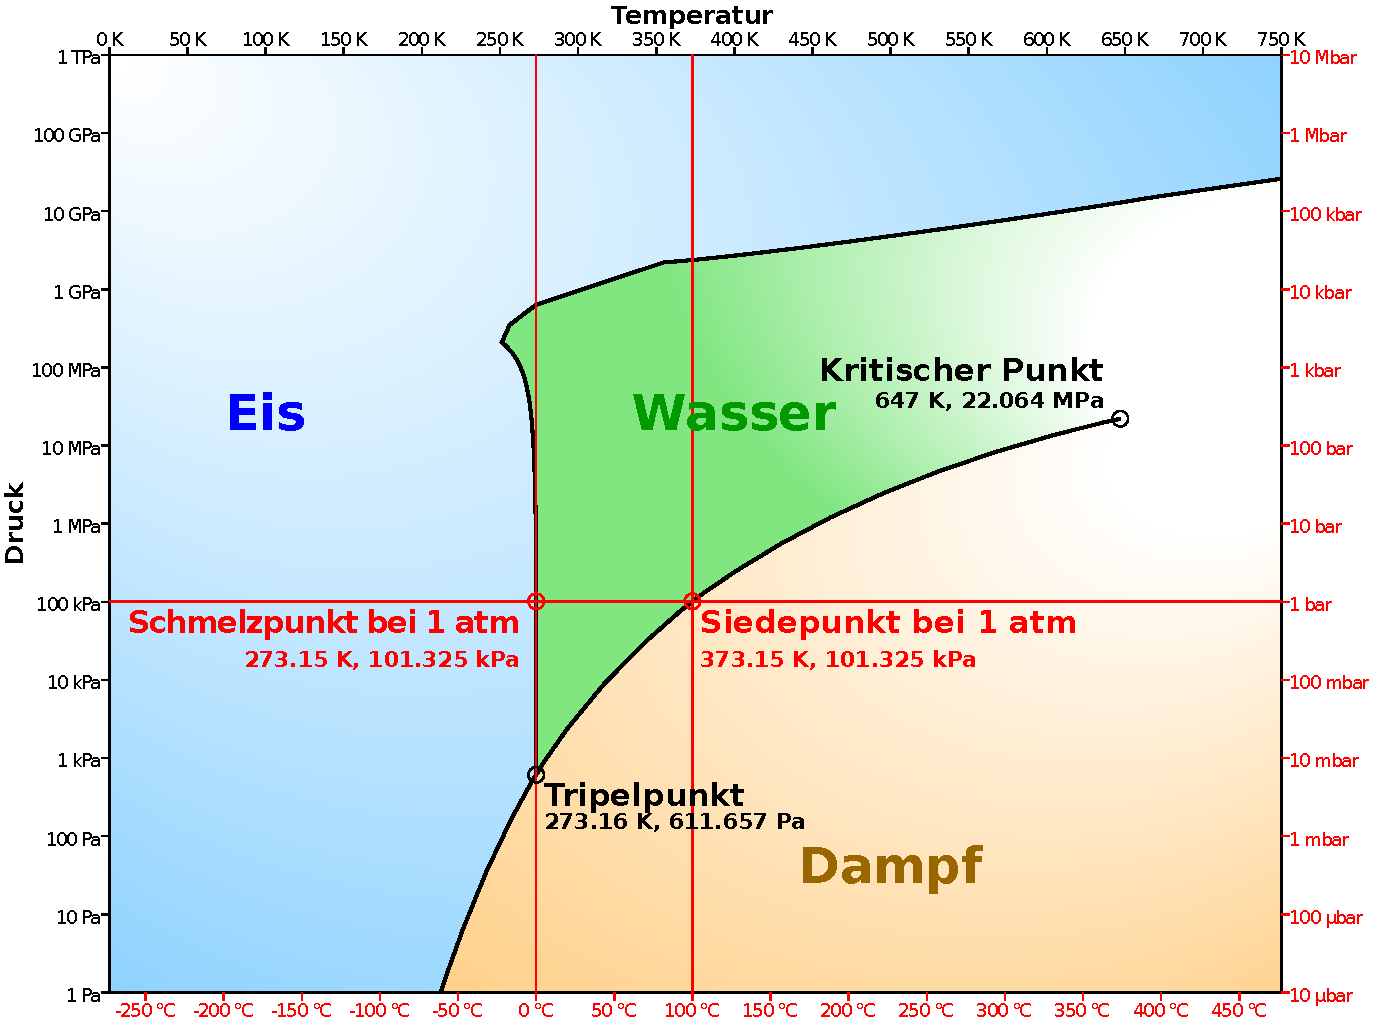
\includegraphics[width=0.7\linewidth]{bilder/Phase_diagram_of_water_simplified.pdf}
		\caption{Phasendiagramm von Wasser, Quelle: Cmglee nach LSBU}
	\end{figure}

	\note{
		%TODO Notizen einfügen
	}
\end{frame}

\begin{frame}
	\frametitle{Interaktion Kryosphäre und Lithosphäre}

	\begin{figure}
		\centering
		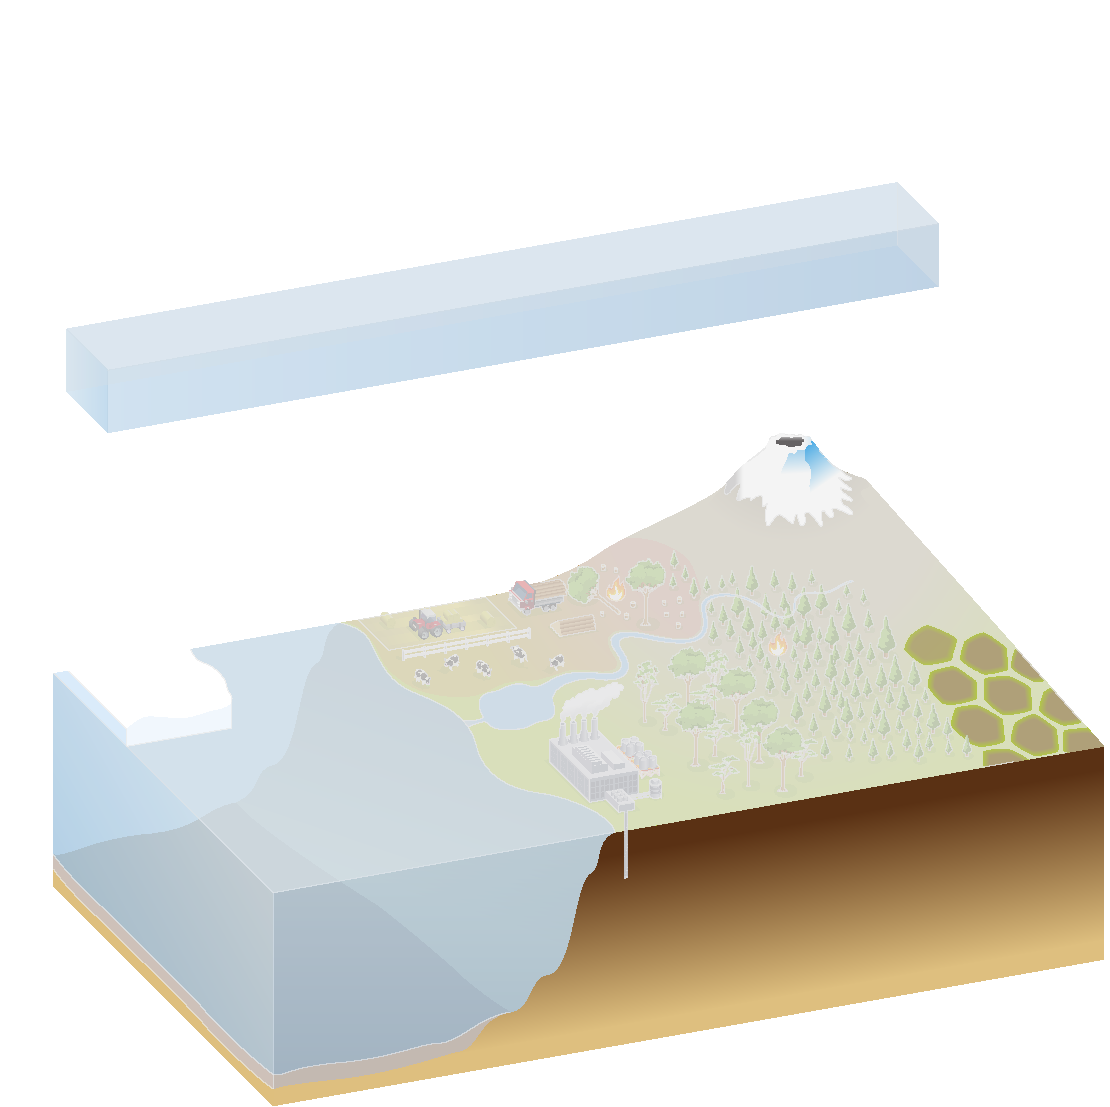
\includegraphics[trim={1cm 0cm 0cm 3cm}, clip, width=0.55\linewidth]{%
				bilder/climate_components/global_climate_components_interaction_kryo_litho.pdf}
		\caption{Interaktion zwischen Kryosphäre und Lithosphäre}
	\end{figure}

	\note{
	\begin{itemize}
		\item[] An der Unterseite des Eisschildes, am Kontakt zwischen Fels und Eis, gibt es einen geothermischen Wärmeeintrag
		\item[$\rightarrow$] Temperatur entlang der Eissäule nimmt mit der Tiefe zu.
		\item[$\rightarrow$] Druckschmelzpunkt kann erreicht werden, sodass flüssiges Wasser an der Grenzschicht vorliegt.
		\item[$\rightarrow$] Schmierfilm, für den Eisschild, der zur schnellen Destabilisierung des westantarktischen Eisschildes führen kann.
		\item[] Weiterhin: Absenkung des Fels durch Gewicht des Eises um etwa \SI{30}{\percent} der Eisdicke
		\item[$\rightarrow$] Nordamerika und Skandinavien heben sich immer noch infolge der Entlastung der eiszeitlichen Eisschilde
	\end{itemize}
	}
\end{frame}
